%!TEX root = ../main.tex

\section{TensorFlow 实战}

\subsection{问题描述}

\begin{frame}{\insertsection}{\insertsubsection}
有 300 个点, 其分布如下图所示, 目标是用一个神经网络, 来拟合这 300 个点.\vspace{10pt}

\begin{tikzpicture}
\begin{axis}[width = \textwidth,
             height = 7cm]
\addplot[only marks] table[col sep = comma] {./data/training_data.dat};
\end{axis}
\end{tikzpicture}
\end{frame}

\subsection{建立网络}
\begin{frame}[fragile]{\insertsection}{\insertsubsection}
我门用一个两层网络来实现对这些离散点的拟合, 这两层网络的公式为:%
%
\begin{flalign*}
  && x_2 &= \textrm{relu}(W_1x_1 + b_1)\text{,} && \text{$W_1\in\mathbb{R}^{10\times1}$, $b_1\in\mathbb{R}^{10\times1}$,} &&\\
  && \hat{y} &= W_2x_2 + b_2\text{,}                  && \text{$W_2\in\mathbb{R}^{1\times10}$, $b_2\in\mathbb{R}^{1\times1}$.} &&
\end{flalign*}

\begin{minipage}[m]{0.38\textwidth}
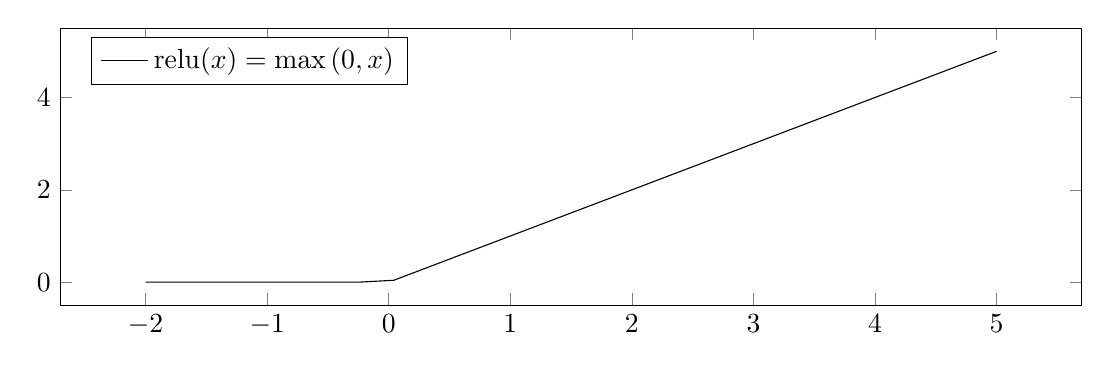
\begin{tikzpicture}
  \begin{axis}[width = 1.2\textwidth,
               height = 5.1cm,
               legend pos = north west,
  ]
    \addplot[mark = none, domain = -2:5] {(x < 0) * 0 + (x >= 0) * x};
    \legend{{$\mathrm{relu}(x) = \max{(0, x)}$}};

  \end{axis}
\end{tikzpicture}
\end{minipage}%
\hfill%
\begin{minipage}[m]{0.60\textwidth}
\begin{pythoncode}
x1 = tf.placeholder(tf.float32, [None, 1])
w1 = tf.Variable(tf.random_normal([1, 10]))
b1 = tf.Variable(tf.ones([1, 10]))

x2 = tf.nn.relu(tf.matmul(x1, w1) + b1)
w2 = tf.Variable(tf.random_normal([10, 1]))
b2 = tf.Variable(tf.ones([1, 1]))
y = tf.matmul(x2, w2) + b2
\end{pythoncode}
\end{minipage}
\end{frame}

\subsection{训练网络}
\begin{frame}[fragile]{\insertsection}{\insertsubsection}
我们用统计学中的均方误差作为代价函数来训练网络, 如下所示.%
%
\[
  \ell(W_1, b_1, W_2, b_2) = \frac{1}{n}\sum_{i = 1}^n (y - \hat{y})^2\text{.}
\]%
%
根据上式可以写出 TensorFlow 中的训练目标.
\begin{pythoncode}
actual_values = tf.placeholder(tf.float32, [None, 1])
loss = tf.reduce_mean(tf.reduce_sum(tf.square(actual_values - y), reduction_indices = [1]))

train_step = tf.train.GradientDescentOptimizer(0.1).minimize(loss)
\end{pythoncode}

我们可以看出, \inlinepython{tf.placeholder} 一般对应着训练数据, 因为训练数据只能在训练的时候给出, 在定义计算图的时候不知道具体的值, \inlinepython{tf.placeholder} 起占位的作用.
\end{frame}

\begin{frame}[fragile]{\insertsection}{\insertsubsection}
训练网络的过程, 就是求使代价函数 $\ell(W_1, b_1, W_2, b_2)$ 达到最小值时的参数集合 $W_1$, $b_1$, $W_2$, $b_2$. 而且需要启动一个会话 \inlinepython{tf.Session} 来完成运算图的计算.

\begin{pythoncode}
session = tf.Session()
session.run(tf.initialize_all_variables())

for step in range(1000):
    feed_dict = {x1:input_data, actual_values:output_data}
    session.run(train_step, feed_dict = feed_dict)

    if step % 50 == 0:
        print(session.run(loss, feed_dict = feed_dict))

session.close()
\end{pythoncode}
\end{frame}

\subsection{测试网络}

\subsection{}